\chapter{Scattering Amplitudes}
In this chapter we derive Feynman's Rules for calculating scattering amplitudes in $\phi^3$ theory. Now that we know that $Z(J)=\exp i W(J)$ we can start to calculate correlation functions and get information from them. For instance, we can check for consistency by evaluating the familar result
\begin{equation}
    \frac{1}{i}\Delta(x_1-x_2)=\vev{\text{T}\phi(x_1)\phi(x_2)}.
\end{equation}
To clear the notation, we introduce $\delta_j=\frac{1}{i}\fdv{J(x_j)}$. Calculating the derivatives, recalling that $Z(0)=1$, gives
\begin{equation}
\begin{aligned}
     \vev{\text{T}\phi(x_1)\phi(x_2)}&= \delta_1\delta_2Z(J)\eval_{J=0}\\
     &=\delta_1[Z(J)\delta_2iW(J)]\eval_{J=0}\\
     &=\delta_1Z(J)\eval_{J=0}\delta_2 iW(J)\eval_{J=0}+Z(J)\delta_1\delta_2iW(J)\eval_{J=0}\\
     &=\delta_1iW(J)\eval_{J=0}\delta_2 iW(J)\eval_{J=0} + \delta_1\delta_2iW(J)\eval_{J=0}.
\end{aligned}
\end{equation}
Since $\delta_jiW(J)\eval_{J=0}=\vev{\phi(x_j)}=0$, then
\begin{equation}
    \vev{\text{T}\phi(x_1)\phi(x_2)}=\delta_1\delta_2iW(J)\eval_{J=0}
\end{equation}
which is the sum of connected diagrams with two sources, but with the two sources removed:
\begin{equation}
    \vev{\text{T}\phi(x_1)\phi(x_2)}=
    \begin{gathered}
       \begin{tikzpicture}
     \draw (0,0) -- (1,0.0);
    \end{tikzpicture}
    \end{gathered}
    +
     \begin{gathered}
       \begin{tikzpicture}
     \draw (0,0) -- (1,0);
     \draw (1.5,0) circle(0.5);
     \draw (2,0) -- (3,0);
    \end{tikzpicture}
    \end{gathered}
    +\order{g^4}
    % \begin{gathered}
     %  \begin{tikzpicture}
     %\draw (0,0) -- (1,0);
     %\draw (1.5,0) circle(0.5);
     %\draw (2,0) -- (3,0);
     %\draw (1.5,-0.5) -- (1.5,0.5);
    %\end{tikzpicture}
    %\end{gathered}
    \label{nao_conectados}
\end{equation}
Which agrees, up to $\order{g^2}$, with what we expected: $\vev{\text{T}\phi(x_1)\phi(x_2)}=\frac{1}{i}\Delta(x_1-x_2)$.\\

We now focus on the object we are most interested in, since it goes into the LSZ formula, the four-point correlation:
\begin{equation}
    \vev{\text{T}\phi(x_1)\phi(x_2)\phi(x_3)\phi(x_4)}=\delta_1\delta_2\delta_3\delta_4 Z(J)\eval_{J=0},
\end{equation}
for which the result is
\begin{equation}
\begin{aligned}
     \vev{\text{T}\phi(x_1)\phi(x_2)\phi(x_3)\phi(x_4)}&=\frac{1}{i}\Delta(x_{1^\prime}-x_2)\frac{1}{i}\Delta(x_{1}-x_{2^\prime})\\&+\frac{1}{i}\Delta(x_{1}-x_2)\frac{1}{i}\Delta(x_{1^\prime}-x_{2^\prime})\\&+\frac{1}{i}\Delta(x_1-x_{1^\prime})\frac{1}{i}\Delta(x_2-x_{2^\prime})\\&+\delta_1\delta_2\delta_3\delta_4 i W(J).
     \label{4pointW}
\end{aligned}
\end{equation}
We argue that only the last term is of any interest for scattering. Let's see why. Plugging any of the  terms consisting of products of propagators into the LSZ, say, the term in the next-to-last line in (\ref{4pointW}), we get
\begin{equation}
    \begin{aligned}
    &i^2\int\dd^4x_1\dd^4x_2\dd^4x_{1^\prime}\dd^4x_{2^\prime}e^{i(k_1x_1+k_2x_2-k^\prime_1x_{1^\prime}-k_{2}^\prime x_{2^\prime}})&\\&\times(-\partial_1^2+m^2)(-\partial_{1^\prime}^2+m^2)\Delta(x_1-x_{1^\prime})(-\partial_2^2+m^2)(-\partial^2_{2^\prime}+m^2)\Delta(x_2-x_{2^\prime}).
    \end{aligned}
    \label{produtoLSZ}
\end{equation}
Working on the first pair of Klein-Gordon differential operators (the other is completely analogous), we define the function $F(x_1-x_{1^\prime})=(-\partial_1^2+m^2)(-\partial_{1^\prime}^2+m^2)\Delta(x_1-x_{1^\prime})$. The product in (\ref{produtoLSZ}) involving this function and the variables it depends on is
\begin{equation}
    \int\dd^4x_1\dd^4x_{1^\prime}e^{i(k_1x_1-k^\prime_1x_{1^\prime})}F(x_1-x_{1^\prime}).
    \label{termoF}
\end{equation}
We change variables to $y=x_1-x_{1^\prime}$ and $z=\frac{1}{2}(x_1+x_{1^\prime})$, so that (\ref{termoF}) reads
\begin{equation}
    \int\abs{\pdv{(x_1,x_{1^\prime})}{(y,z)}}\dd^4y\,\dd^4z\,e^{i(k_1+k_1^\prime)y/2}e^{i(k_1-k_1^\prime)z}F(y)
\end{equation}
since the jacobian for such transformation of variables is $1$, we see that 
\begin{equation}
    \int\dd^4x_1\dd^4x_{1^\prime}e^{i(k_1x_1-k^\prime_1x_{1^\prime})}F(x_1-x_{1^\prime})
    =(2\pi)^4\delta^4(k_1-k_1^\prime)\widetilde{F}(\Bar{k}_{11})
\end{equation}
where $\widetilde{F}(\Bar{k}_{11})$ is the Fourier transform of $F(y)$ and $\bar{k}_{ij}=\frac{1}{2}(k_i+k_j^\prime)$.
Therefore, (\ref{produtoLSZ}) gives the following contribution to the amplitude
\begin{equation}
\braket{f}{i}=i^2(2\pi)^4\delta^4(k_1-k_{1^\prime})(2\pi)^4\delta^4(k_2-k_{2^\prime})\widetilde{F}(\bar{k}_{11})\widetilde{F}(\bar{k}_{22})
\end{equation}
which is a selection rule for processes in which the 4-momentum of the particles do not change in transitioning from the in and out states: they do not correspond to a scattering. We conclude then that terms involving the product of propagators in (\ref{4pointW}) do not contribute to scattering, either because of what we just presented or because they vanish, since some of them can involve $\delta^4(k_1+k_2)$ or $\delta^4(k_1^\prime+k_2^\prime)$. As a result, since the sum of energies is always positive, i.e. $k_1^0+k_2^0\geq2m>0$, we never reach the ``peak" of the Delta distribution: integrals involving these Deltas vanish.\\

Therefore, products of diagrams such as the ones in (\ref{nao_conectados}) do not contribute to scattering amplitudes. 
%The only term contributing is the last one in (\ref{4pointW})), which corresponds to the sum of connected diagrams with four sources, with those sources removed, that is ().
This motivates the definition of a \textit{fully connected correlation function} as the term that actually contributes to scattering
\begin{equation}
    \vev{\text{T}\phi(x_1)\dots\phi(x_E)}_{\text{C}}=\delta_1\delta_2\dots\delta_EiW(J)\eval_{J=0}.
\end{equation}
The term we are interested in, $\delta_1\delta_2\delta_3\delta_4 i W(J)$, when $J=0$, corresponds to the sum of diagrams with four sources, but with them removed. Up to $g^2$, we highlight the diagram of interest in (\ref{iWphi3}).
\begin{equation}
iW(J)=\dots+
\begin{gathered}
              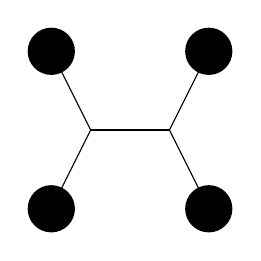
\begin{tikzpicture}
                \fill[black] (1,1) circle (0.3 cm);
                 \fill[black] (-1,1) circle (0.3 cm);
                 \fill[black] (-1,-1) circle (0.3cm);
                 \fill[black] (1,-1) circle (0.3 cm);
                 \draw (-0.5,0) -- (0.5,0);
                 \draw (-1,1) -- (-0.5,0);
                 \draw (1,1) -- (0.5,0);
                 \draw (-1,-1) -- (-0.5,0);
                 \draw (1,-1) -- (0.5,0);
            \end{tikzpicture}
\end{gathered}+\order{g^4}
\label{tree_sources}
\end{equation}
This diagram with its sources removed will consist of different arrangements of labels $x_i$, due to the possible actions of the functional derivatives. There are $4!$ of such arrangements and they are exactly eight copies of the same three diagrams below, called \textit{tree diagrams}
\begin{equation}
\delta_1\delta_2\delta_3\delta_4 i W(J)=
\begin{gathered}
    \begin{tikzpicture}
     \feynmandiagram [small,horizontal=a to b] {
      i1 [particle=\(x_2\)] --  a --  i2 [particle=\(x_1\)],
      a --  b,
      f1 [particle=\(x_{2^\prime}\)] --  b --  f2 [particle=\(x_{1^\prime}\)],
    };
    \end{tikzpicture}
\end{gathered}+
\begin{gathered}
    \feynmandiagram [small,vertical=a to b] {
      i1 [particle=\(x_1\)] --  a --  i2 [particle=\(x_{1^\prime}\)],
      a --  b,
      f1 [particle=\(x_2\)] --  b --  f2 [particle=\(x_{2^\prime}\)],
    };
\end{gathered}+
\begin{gathered}
   \feynmandiagram [small,vertical=a to b] {
      i1 [particle=\(x_1\)] --  a --  i2 [particle=\(x_{2^\prime}\)],
      a --  b,
      f1 [particle=\(x_2\)] --  b --  f2 [particle=\(x_{1^\prime}\)],
    };
\end{gathered} +\order{g^4}
\label{trees}
\end{equation}
Since the diagram highlighted in (\ref{tree_sources}) has symmetry factor $S=8$, the eight copies of the three configurations cancel the symmetry factor. Tree-diagrams thus have this property: after removing the sources, we get $S=1$ for their symmetry factor. Translating (\ref{trees}) we find
\begin{equation}
\begin{aligned}
  \vev{\text{T}\phi(x_1)\phi(x_2)\phi(x_1^\prime)\phi(x_2^\prime)}_{\text{C}}&=(ig)^2\qty(\frac{1}{i})^5\int\dd^4 y\,\dd^4 z\, \Delta(y-z)\\
  &\times[\Delta(x_1-y)\Delta(x_2-y)\Delta(x_{1^\prime}-z)\Delta(x_{2^\prime}-z)\\
  &+\Delta(x_1-y)\Delta(x_{1^\prime}-y)\Delta(x_2-z)\Delta(x_{2^\prime}-z)\\
  &+\Delta(x_1-y)\Delta(x_{2^\prime}-y)\Delta(x_2-z)\Delta(x_{1^\prime}-z)]+\order{g^4}
\end{aligned}
\end{equation}
Plugging in the LSZ, bearing in mind that the propagator $\Delta(x-y)$ is the Green's Function for the Klein-Gordon differential operator $(-\partial^2+m^2)$, we have
\begin{equation}
\begin{aligned}
   \braket{f}{i}&=i^4\int\dd^4x_1\dd^4x_2\dd^4x_{1^\prime}\dd^4x_{2^\prime}\,e^{ik_1x_1}e^{ik_2x_2}e^{-ik_{1}^\prime x_{1^\prime}}e^{-ik_{2}^\prime x_{2^\prime}}\\&\qquad\quad\times(-\partial_1^2+m^2)(-\partial_2^2+m^2)
    \,(-\partial_{1^\prime}^2+m^2)(-\partial_{2^\prime}^2+m^2)\\&\qquad\quad\times\bra{0}\text{T}\phi(x_1)\phi(x_2)\phi(x_{1^\prime})\phi(x_{2^\prime})\ket{0}_{\text{C}}\\
    &=(ig)^2\frac{1}{i}\int\dd^4y\,\dd^4z\,\dd^4x_1\,\dd^4x_2\,\dd^4x_{1^\prime}\,\dd^4x_{2^\prime}\, e^{i(k_1x_1+k_2x_2-k_1^\prime x_{1^\prime} - k_2^\prime x_{2^\prime})}\Delta(y-z)\\
    &\qquad\quad\times\Big{[}\delta^4(x_1-y)\delta^4(x_2-y)\delta^4(x_{1^\prime}-z)\delta^4(x_{2^\prime}-z)\\
  &\qquad\quad+\delta^4(x_1-y)\delta^4(x_{1^\prime}-y)\delta^4(x_2-z)\delta^4(x_{2^\prime}-z)\\
  &\qquad\quad+\delta^4(x_1-y)\delta^4(x_{2^\prime}-y)\delta^4(x_2-z)\delta^4(x_{1^\prime}-z)\Big{]}+\order{g^4}\\
  &=ig^2\int\dd^4y\,\dd^4z\,\Delta(y-z)\Big{[}e^{i(k_1y+k_2y-k_1^\prime z -k_2^\prime z)}+e^{i(k_1y+k_2z-k_1^\prime y -k_2^\prime z)}  \\&\qquad\quad + e^{i(k_1y+k_2z-k_1^\prime z - k_2^\prime y)}\Big{]}+\order{g^4}.
\end{aligned}
\end{equation}
We use the definition of the propagator
\begin{equation}
    \Delta(y-z)=\int\frac{\dd ^4 k}{(2\pi)^4}\frac{e^{ik(y-z)}}{k^2+m^2-i\epsilon}
\end{equation}
and the Dirac Delta 
\begin{equation}
    \delta^4(w-v)=\int\frac{\dd^4 k}{(2\pi)^4}e^{i(w-v)k}
\end{equation}
so the amplitude reads
\begin{equation}
\begin{aligned}
   \braket{f}{i}=&ig^2\int\frac{\dd^4 k}{(2\pi)^4}\frac{1}{k^2+m^2-i\epsilon}\Big{[}(2\pi)^4\delta^4(k_1+k_2+k)(2\pi)^4\delta^4(k_1^\prime+k_2^\prime+k)\\
   &+(2\pi)^4\delta^4(k_1-k_1^\prime+k)(2\pi)^4\delta^4(k_2^\prime-k_2+k)\\&+(2\pi)^4\delta^4(k_1-k_2^\prime+k)(2\pi)^4\delta^4(k_1^\prime-k_2+k)\Big{]}+\order{g^4}
\end{aligned}
\end{equation}
and we finally arrive at
\begin{equation}
\begin{aligned}
    \braket{f}{i}=&ig^2(2\pi)^4\delta^4(k_1+k_2-k_1^\prime-k_2^\prime)\\
    &\times\qty[\frac{1}{(k_1+k_2)^2+m^2}+\frac{1}{(k_1-k_1^\prime)^2+m^2}+\frac{1}{(k_1-k_2^\prime)^2+m^2}]+\order{g^4}
    \label{fi_final},
\end{aligned}
\end{equation}
where we dropped the $i\epsilon$s since the denominators cannot vanish for physically allowed values of momenta. This result can be generalized as
\begin{equation}
    \braket{f}{i}=(2\pi)^4\delta^4(k_{\text{in}}-k_{\text{out}})i\mathcal{T}
    \label{scattering_amplitude}
\end{equation}
in which the $i\mathcal{T}$ will be determined according to \textit{Feynman's Rules}. These rules allow us to translate diagrams directly into scattering amplitudes, without repeating  the previous calculations we have done.
The Feynman Rules for $\phi^3$ theory are
\begin{itemize}
    \item We draw lines for incoming and outgoing particles. Time runs from left to right.
    \item One side of these incoming and outgoing lines must be free while the other must be joined to a \textit{vertex}. A vertex must join three lines. We must draw all the \textit{topologically nonequivalent} diagrams: those that cannot be transformed into another one by deformations.
    \item For each incoming line, draw an arrow pointing toward the vertex; for each outgoing line draw an arrow pointing outward the vertex; for internal lines draw an arrow with arbitrary direction.
    \item To each line, associate a 4-momentum. To external lines, this 4-momentum should be that of the particle the line represents
    \item Think of 4-momentum as a fluid flowing through the diagram and demand its conservation at the vertices.
    \item When translating into scattering amplitudes, external lines equals to $1$.
    \item Internal lines with 4-momentum $k$ correspond to $\frac{-i}{k^2+m^2-i\epsilon}$
    \item Vertices correspond to $iZ_gg$.
\end{itemize}
This way,  result (\ref{fi_final}) we found can be stated as (\ref{scattering_amplitude}) where
\begin{equation}
    i\mathcal{T}=
    \begin{gathered}
       \feynmandiagram [medium,horizontal=a to b] {
      i1 [particle=\(k_2\)] -- [fermion]  a -- [anti fermion] i2 [particle=\(k_1\)],
      a -- [momentum=\(k_1+k_2\)] b,
      f1 [particle=\(k_{1}^\prime\)] -- [anti fermion]  b -- [fermion]  f2 [particle=\(k_{2}^\prime\)],
    };
    \end{gathered}+
    \begin{gathered}
       \feynmandiagram [medium,vertical=a to b] {
      i1 [particle=\(k_1\)] -- [fermion]  a -- [fermion] i2 [particle=\(k_1^\prime\)],
      a -- [momentum=\(k_1-k_1^\prime\)] b,
      f1 [particle=\(k_{2}^\prime\)] -- [anti fermion]  b -- [anti fermion]  f2 [particle=\(k_{2}\)],
    };
    \end{gathered}+
    \begin{gathered}
       \feynmandiagram [medium,vertical=a to b] {
      i1 [particle=\(k_1\)] -- [fermion]  a -- [fermion] i2 [particle=\(k_2^\prime\)],
      a -- [momentum=\(k_1-k_2^\prime\)] b,
      f1 [particle=\(k_{1}^\prime\)] -- [anti fermion]  b -- [anti fermion]  f2 [particle=\(k_{2}\)],
    };
    \end{gathered}
\end{equation}

